\section*{Image Enhancement}

Two broad categories:

\begin{itemize}
  \item \textbf{Spatial Domain:} Direct manipulation of pixels.
  \item \textbf{Frequency Domain:} Manipulation of fourier/wavelet
    transforms of images.
\end{itemize}

\section*{Spatial Domain}

\subsection*{Image Histogram}

Shows the \textbf{distribution of pixel intensities} in an image.
Massively useful, especially for segmentation.

\begin{figure}[H]
  \centering
  \raisebox{-0.5\height}{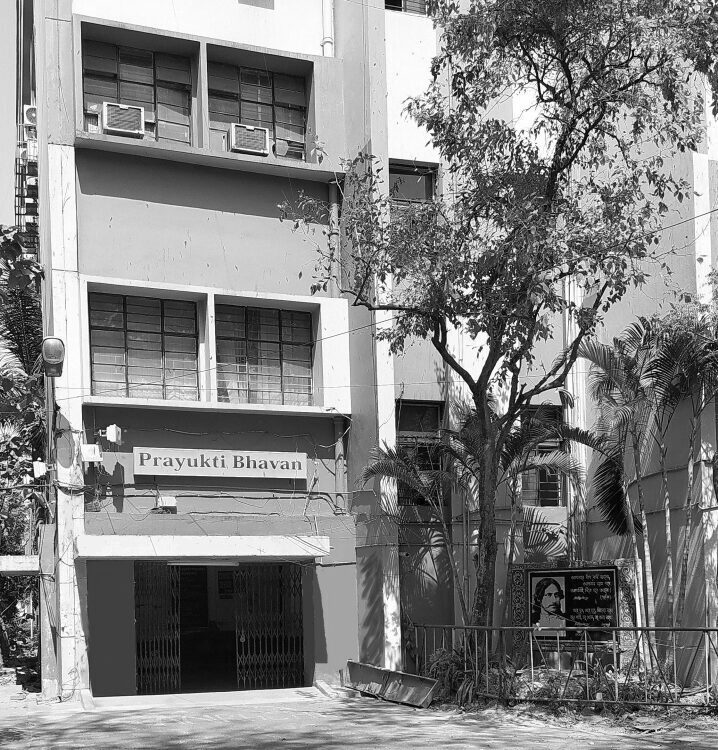
\includegraphics[width=0.3\linewidth]{images/prayukti.jpg}}
  \raisebox{-0.55\height}{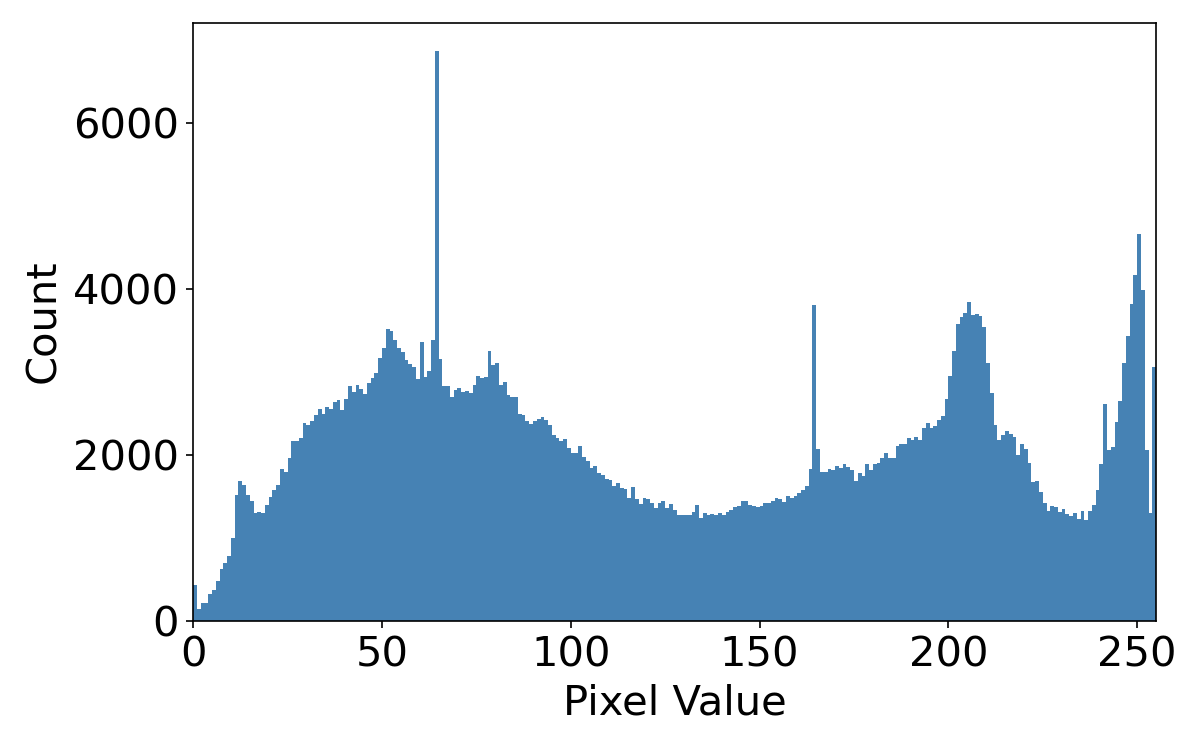
\includegraphics[width=0.6\linewidth]{images/prayukti_histogram.png}}
  \caption{Example image and its histogram}
\end{figure}

\subsection*{Contrast Stretching}

Contrast stretching (normalization) linearly expands an image’s
dynamic range, making low-contrast images more vivid. It’s the
simplest boost, though it can exaggerate noise or outliers.

\begin{equation*}
  s_k = T(r_k)
  = \frac{r_k - r_{\min}}{r_{\max} - r_{\min}}
  \times (L - 1)
\end{equation*}

where: (i) $r_k\rightarrow$ input intensity, (ii) $s_k\rightarrow$
output intensity, (iii) $r_{\min},\,r_{\max}\rightarrow$ observed
minimum and maximum intensities in the image, (iv) $L\rightarrow$
number of possible intensity levels

\begin{algorithm}[ht!]
  \DontPrintSemicolon
  Find $r_{\min}$ and $r_{\max}$ in input image $I$ \;
  {
    \ForEach{\textnormal{pixel intensity} $r_k \in I$}{
      $s_k \leftarrow \bigl(r_k -
      r_{\min}\bigr)\,/\,\bigl(r_{\max}-r_{\min}\bigr)\times(L-1)$ \;
      Clip $s_k$ to $[0,\,L-1]$ \;
    }
  }
  Return contrast-stretched image $I'$\;
  \caption{Contrast Stretching}
\end{algorithm}

\subsection*{Histogram Equalization}

Refers to \enquote{spreading out} (equalizing) the frequencies in an
image. Simple way to improve dark or washed out images.

\begin{equation*}
  s_k = T(r_k) = \sum_{j=1}^{k} p_r(r_j) = \sum_{j=1}^{k} \frac{n_j}{n}
\end{equation*}

where: (i) $r_k \rightarrow$ input intensity, (ii) $s_k \rightarrow$
processed intensity, (iii) $k \rightarrow$ intensity range (e.g. 0 -
1), (iv) $n_j \rightarrow$ frequency of intensity $j$, (v) $n
\rightarrow$ total number of pixels (v) $L\rightarrow$ number of
possible intensity levels

\begin{algorithm}[ht!]
  \DontPrintSemicolon
  Compute histogram of input image $I$ \;
  Compute CDF from histogram \;
  Normalize CDF by dividing by $n$ \;

  {
    Apply $T$ to each pixel intensity $r_k$ in $I$\\
    \nonl $s_k = \text{CDF}[r_k] \times (L - 1)$ \\
    \nonl where $L$ is the number of intensity levels \;
  }

  Return enhanced image $I'$\;
  \caption{Histogram Equalization}
\end{algorithm}

\subsection*{Point Processing}

Simplest spatial domain operation, neighborhood is the pixel itself.

\subsubsection*{Negative Images}

Simply inverts pixel values; useful for enhancing dark regions.
\begin{equation*}
  s = (L - 1) - r
\end{equation*}

\subsubsection*{Thresholding}

Segments an image by \textbf{converting it to binary} based on a
threshold value (say $\theta_0$); useful for isolating objects from
the background.

\begin{equation*}
  s =
  \begin{cases}
    0 & \text{if } r < \theta_0 \\
    L - 1 & \text{if } r \geq \theta_0
  \end{cases}
\end{equation*}

\subsubsection*{Gray Level Transforms}

\begin{figure}[H]
  \centering
  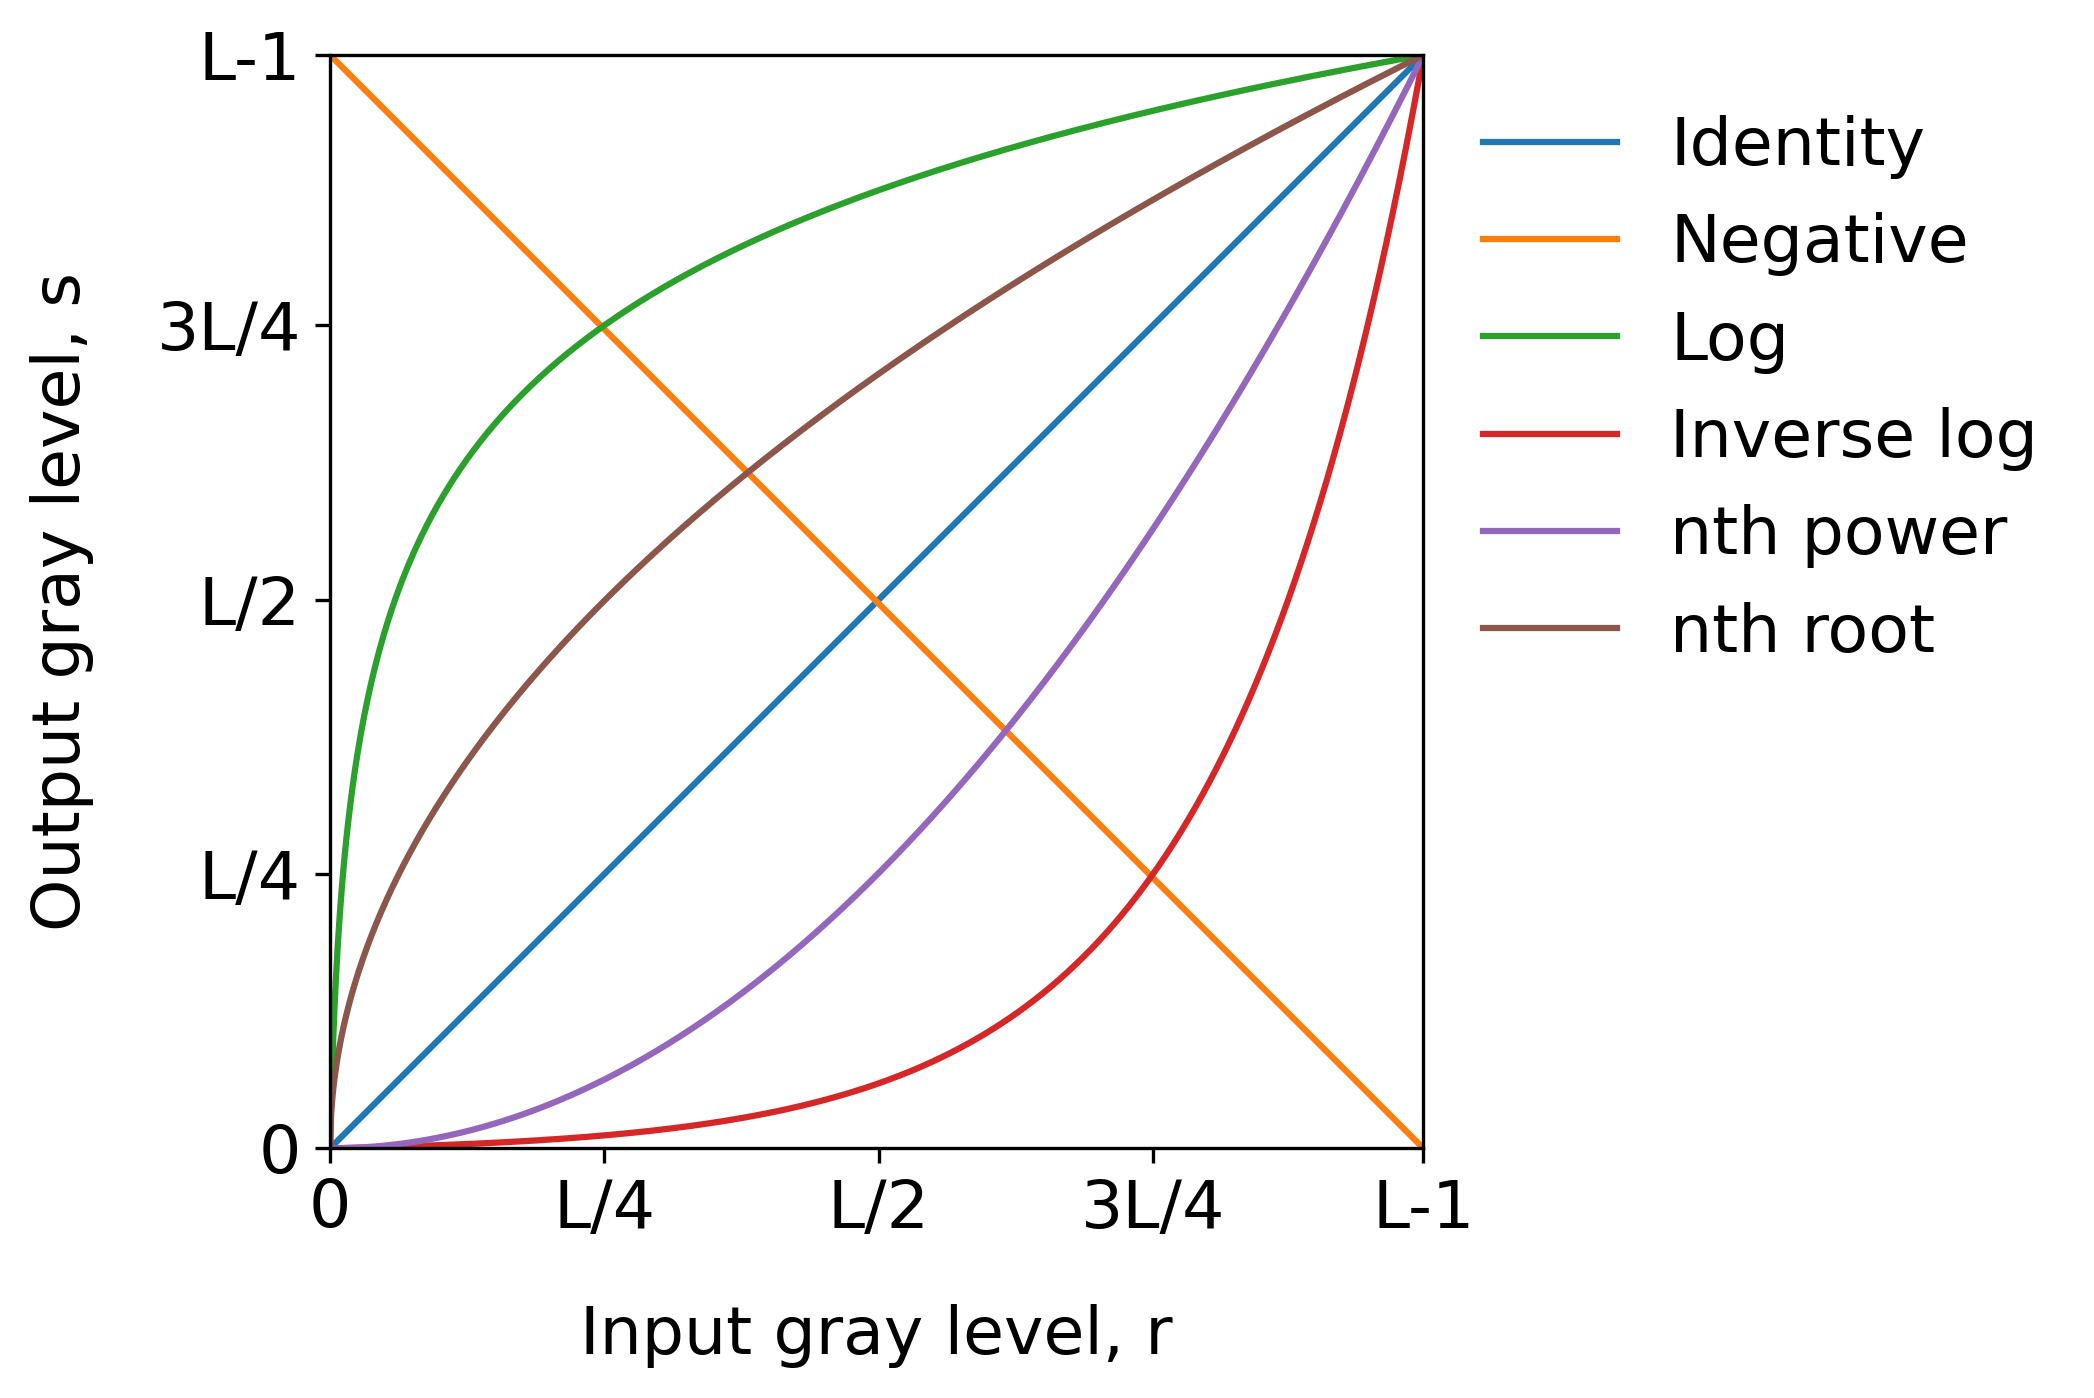
\includegraphics[width=\linewidth]{images/gray_level_transforms.png}
  \caption{Gray level transforms}
\end{figure}

\begin{itemize}
  \item \textbf{Log Transform:} Maps a narrow range of low input grey
    level values into a wider range of output values.
    \begin{itemize}
      \item $s = c \times \log(1 + r)$, where $c$ is a constant
      \item Useful when the input grey level values may have an
        extremely large range of values
      \item Use case 1: \textbf{log transform on Fourier transform}.
        More details are revealed.
      \item Use case 2: \textbf{gamma correction in displays}. Some
        displays do not respond linearly to different intensities;
        can be corrected using log transform
    \end{itemize}

  \item \textbf{Power Law Transform:} Maps a narrow range of dark
    input grey level values into a wider range of output values.
    \begin{itemize}
      \item $s = c \times r^{\gamma}$, where $\gamma$ is a constant
      \item Different $\gamma$ values highlight different details
      \item Useful for enhancing images with high dynamic range
    \end{itemize}

  \item \textbf{Piecewise Linear Transform:} Combines multiple
    arbitrary user-defined linear segments to create a more complex mapping.
    \begin{itemize}
      \item Useful for enhancing specific ranges of pixel values
      \item Can be used to adjust contrast in specific regions of an image
    \end{itemize}

    \begin{minipage}{\linewidth}
      \vspace{-0.5cm}
      \begin{figure}[H]
        \centering
        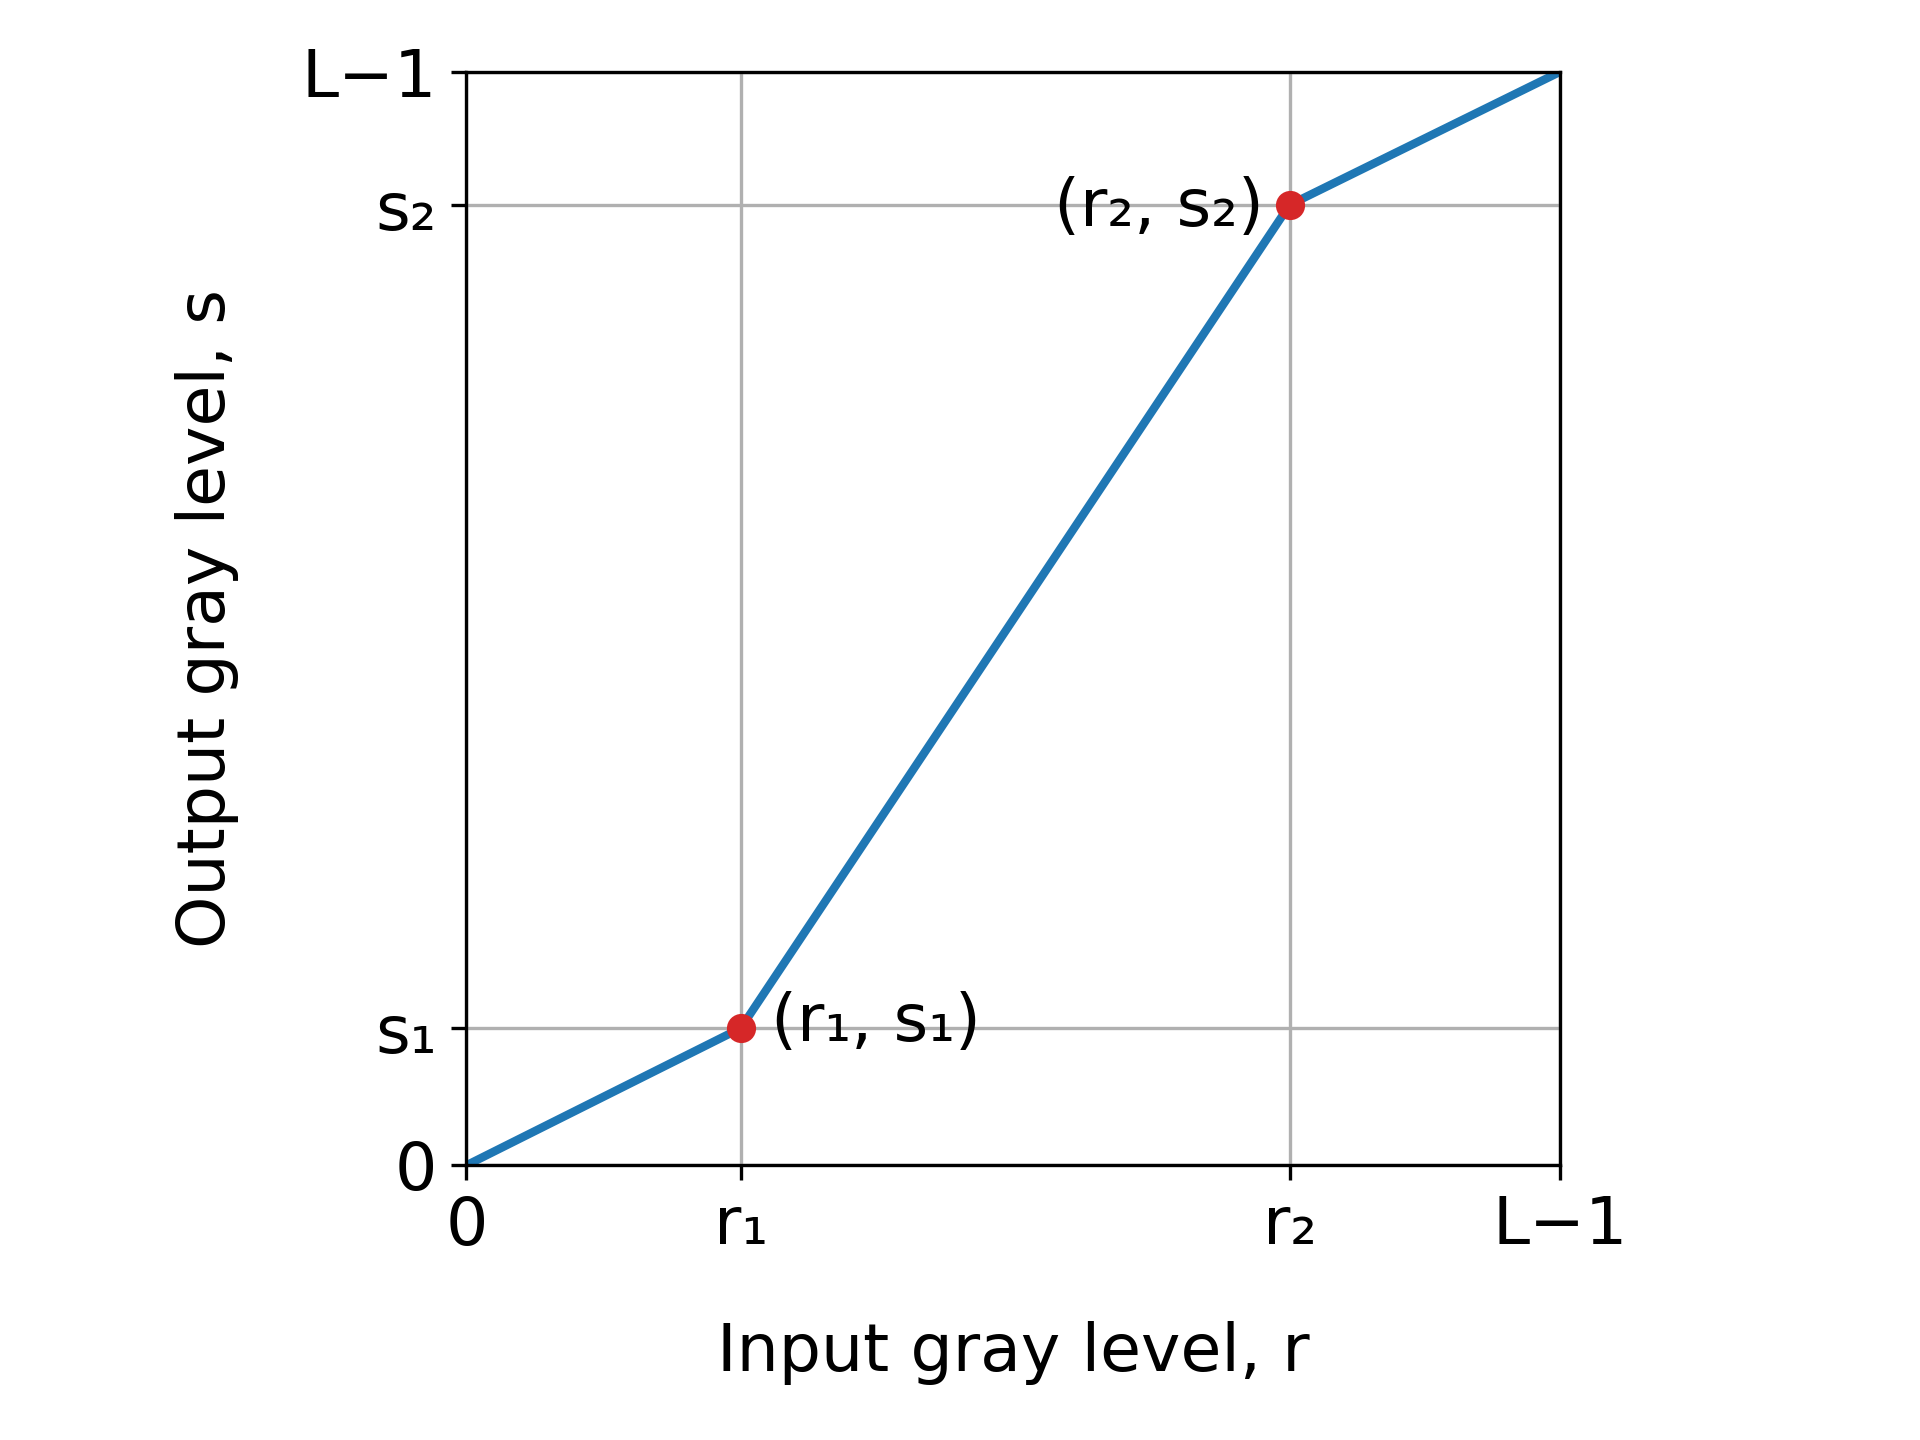
\includegraphics[width=\linewidth]{images/piecewise_transform.png}
        \vspace{-0.5cm}
        \caption{Piecewise linear transform}
      \end{figure}
    \end{minipage}

  \item \textbf{Gray Level Slicing:} Similar to thresholding, but
    allows for a range of pixel values to be highlighted.
    \begin{itemize}
      \item Other levels can be suppressed or maintained
      \item Useful for enhancing specific features in an image
    \end{itemize}

    \begin{figure}[H]
      \centering
      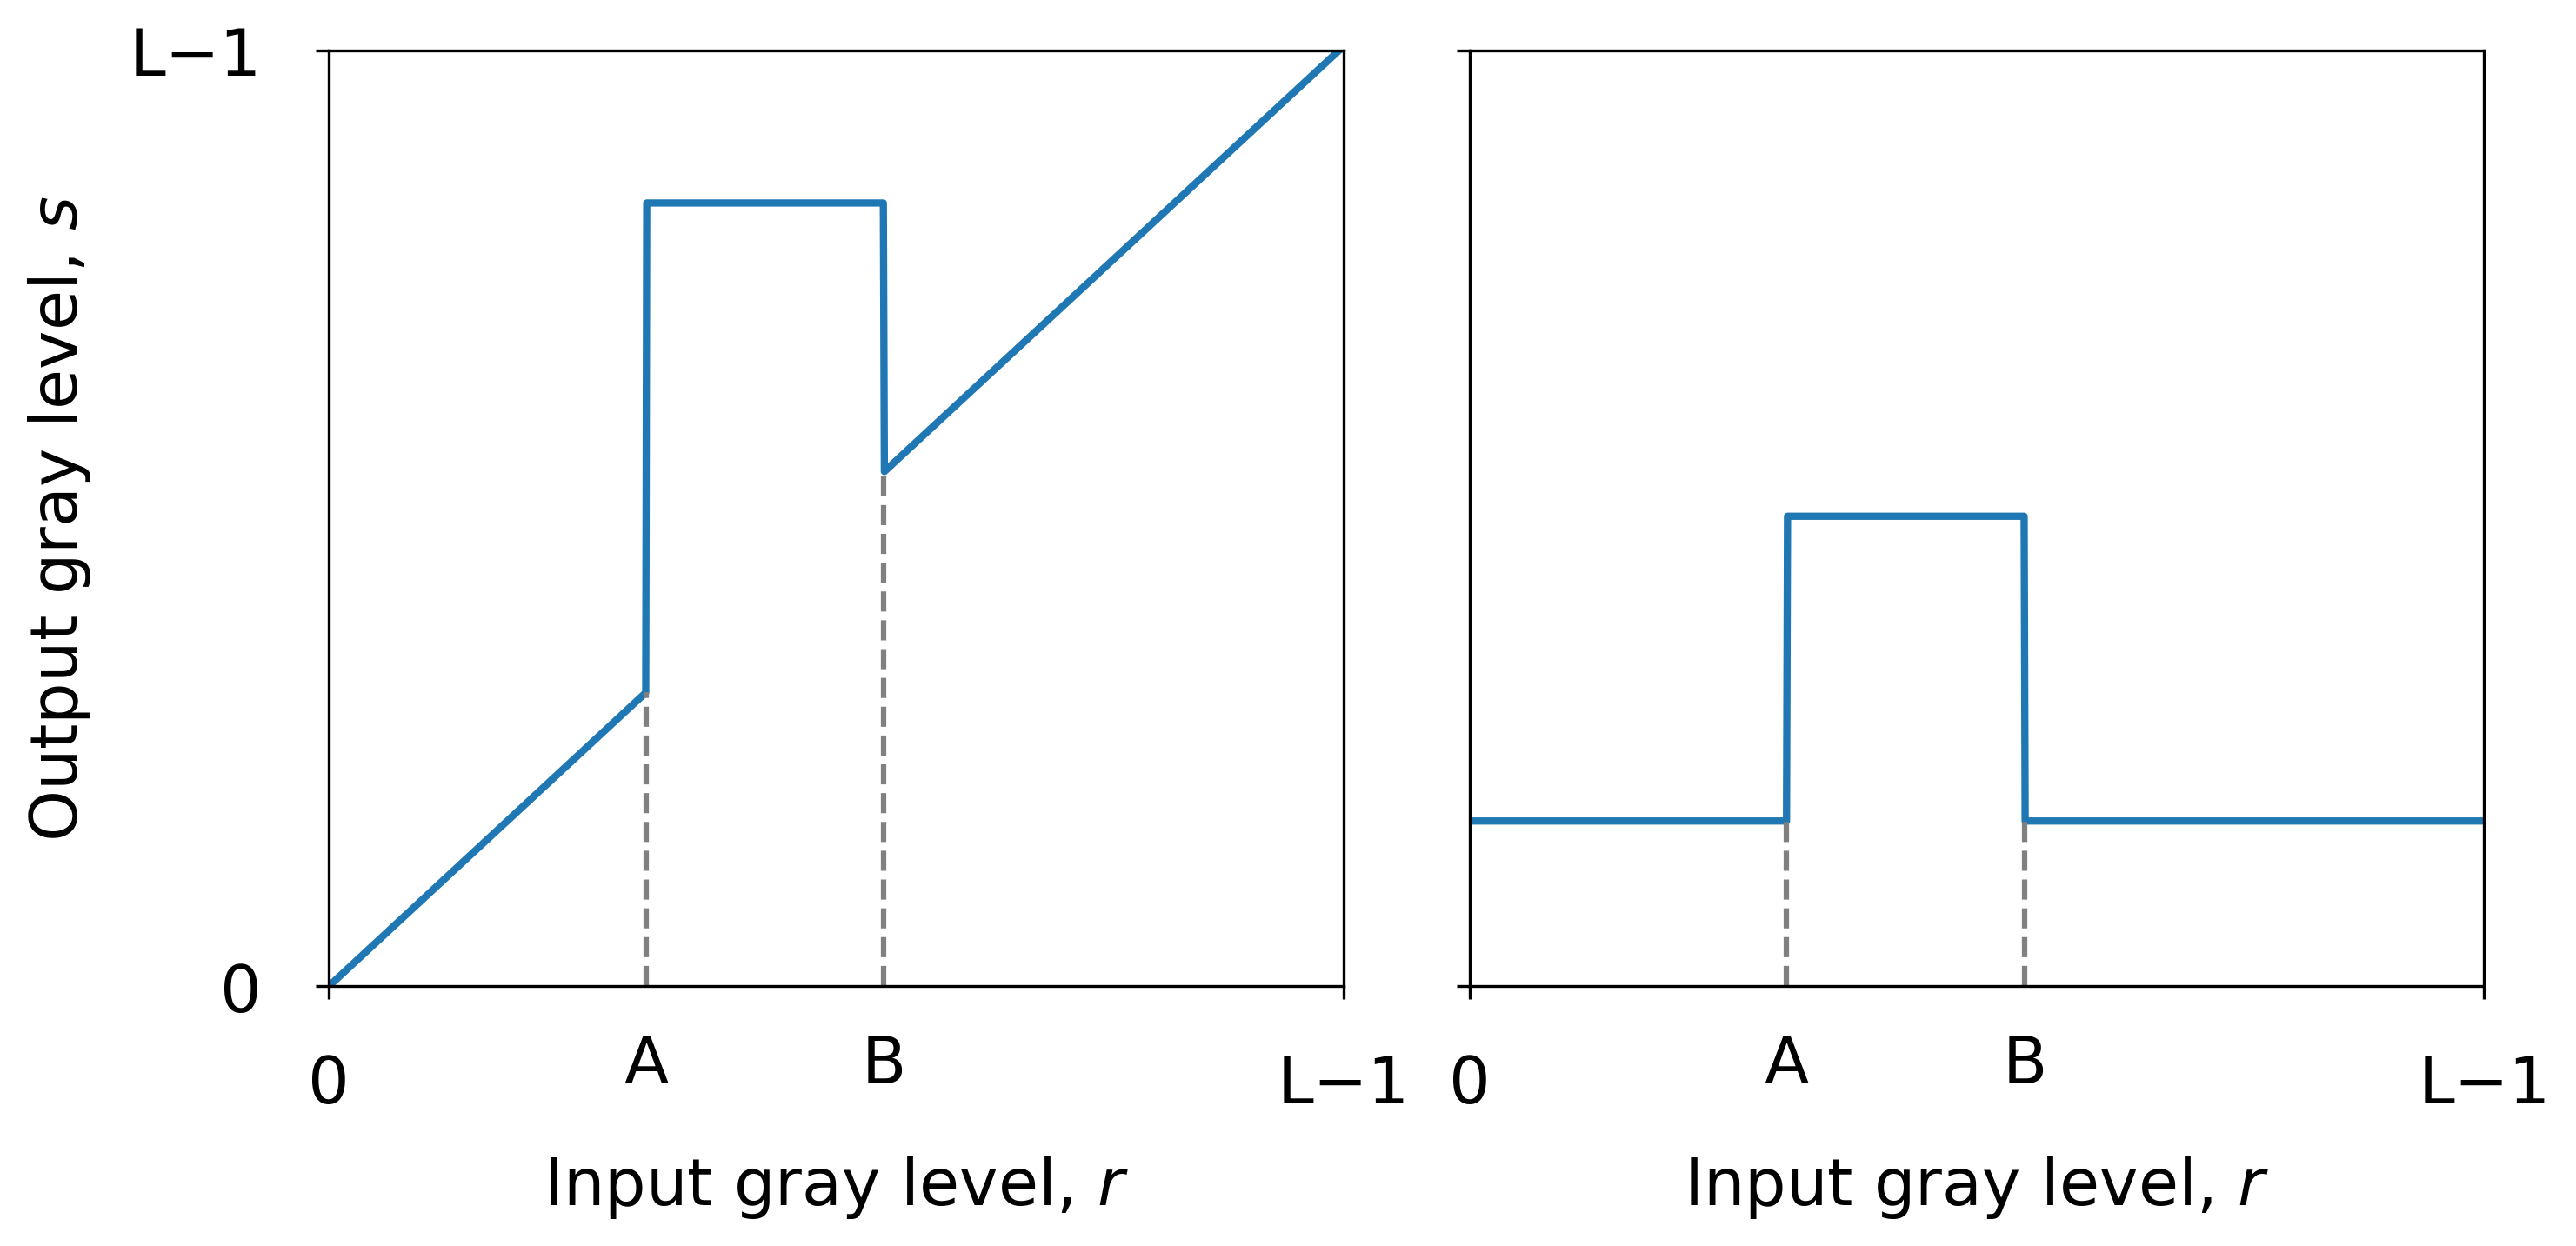
\includegraphics[width=\linewidth]{images/gray_level_slicing.png}
      \caption{Gray level slicing with (i) background retained (ii)
      background supressed}
    \end{figure}

  \item \textbf{Bit-Plane Slicing:} By isolating particular bits of
    the pixel values in an image, we can highligh interesting aspects
    of that image.
    \begin{itemize}
      \item Higher order bits contain most of the significant information
      \item Lower order bits contain subtle details
      \item \enquote{Bit planes} are arranged in a stack; MSB at the
        top, LSB at the bottom. For 8-bit images, top to bottom are
        bit planes 7 to 0.
    \end{itemize}

\end{itemize}
